%%%%%%%%%%%%%%%%%%%%%%%%%%%%%%%%%%%%%%%%%%%%%%%%%%
\chapter{Design and implementation}
\label{chap:design-and-implementation}

This chapter describes the architecture and implementation of the EGR project. The general three phases for gesture recognition, namely tracking, pose estimation and gesture classification, represents also the basis for this project (see chapter \ref{chap:gesture-recognition}). Using the camera, the glove and the software libraries presented in chapter \ref{chap:setup-and-frameworks}, an architecture that aims at recognizing the gestures chosen in chapter \ref{chap:chosen-gestures} is presented in section \ref{sec:architecture}. In the sections \ref{sec:tracker-configuration}, \ref{sec:model-mapping} and \ref{sec:training-and-classification} implementation details of the tracking phase, the pose estimation phase and the classification phase are presented.

%%%-%-%-%-%-%-%-%-%-%-%-%%-%-%-%-%-%-%-%-%-%-%-%%%
\section{Architecture}
\label{sec:architecture}

The separation of the three gesture recognition phases into separate but linked modules allows a better understanding of the mechanisms involved and offers the possibility to replace a module by an alternate future version, which accomplishes the same task. 
There are two main modules and three applications: 
\begin{itemize}
	\item Tracking module
	\item Model module
	\item Recorder application
	\item Training application
	\item Demo application
\end{itemize}

The tracking module is implemented as a C library, which runs a continuous loop in a thread, and performs the image transformations and blob detection algorithms for each new frame from a video source. The hand model module is implemented as a C++ class object, which maps the information obtained from the tracker in a defined structure and optionally can classify a posture, assuming a decision function obtained from the training application is present. This hand object can then be directly instantiated in a potential gesture recognition application and initialized with the necessary information.


\begin{figure}[H]
\center
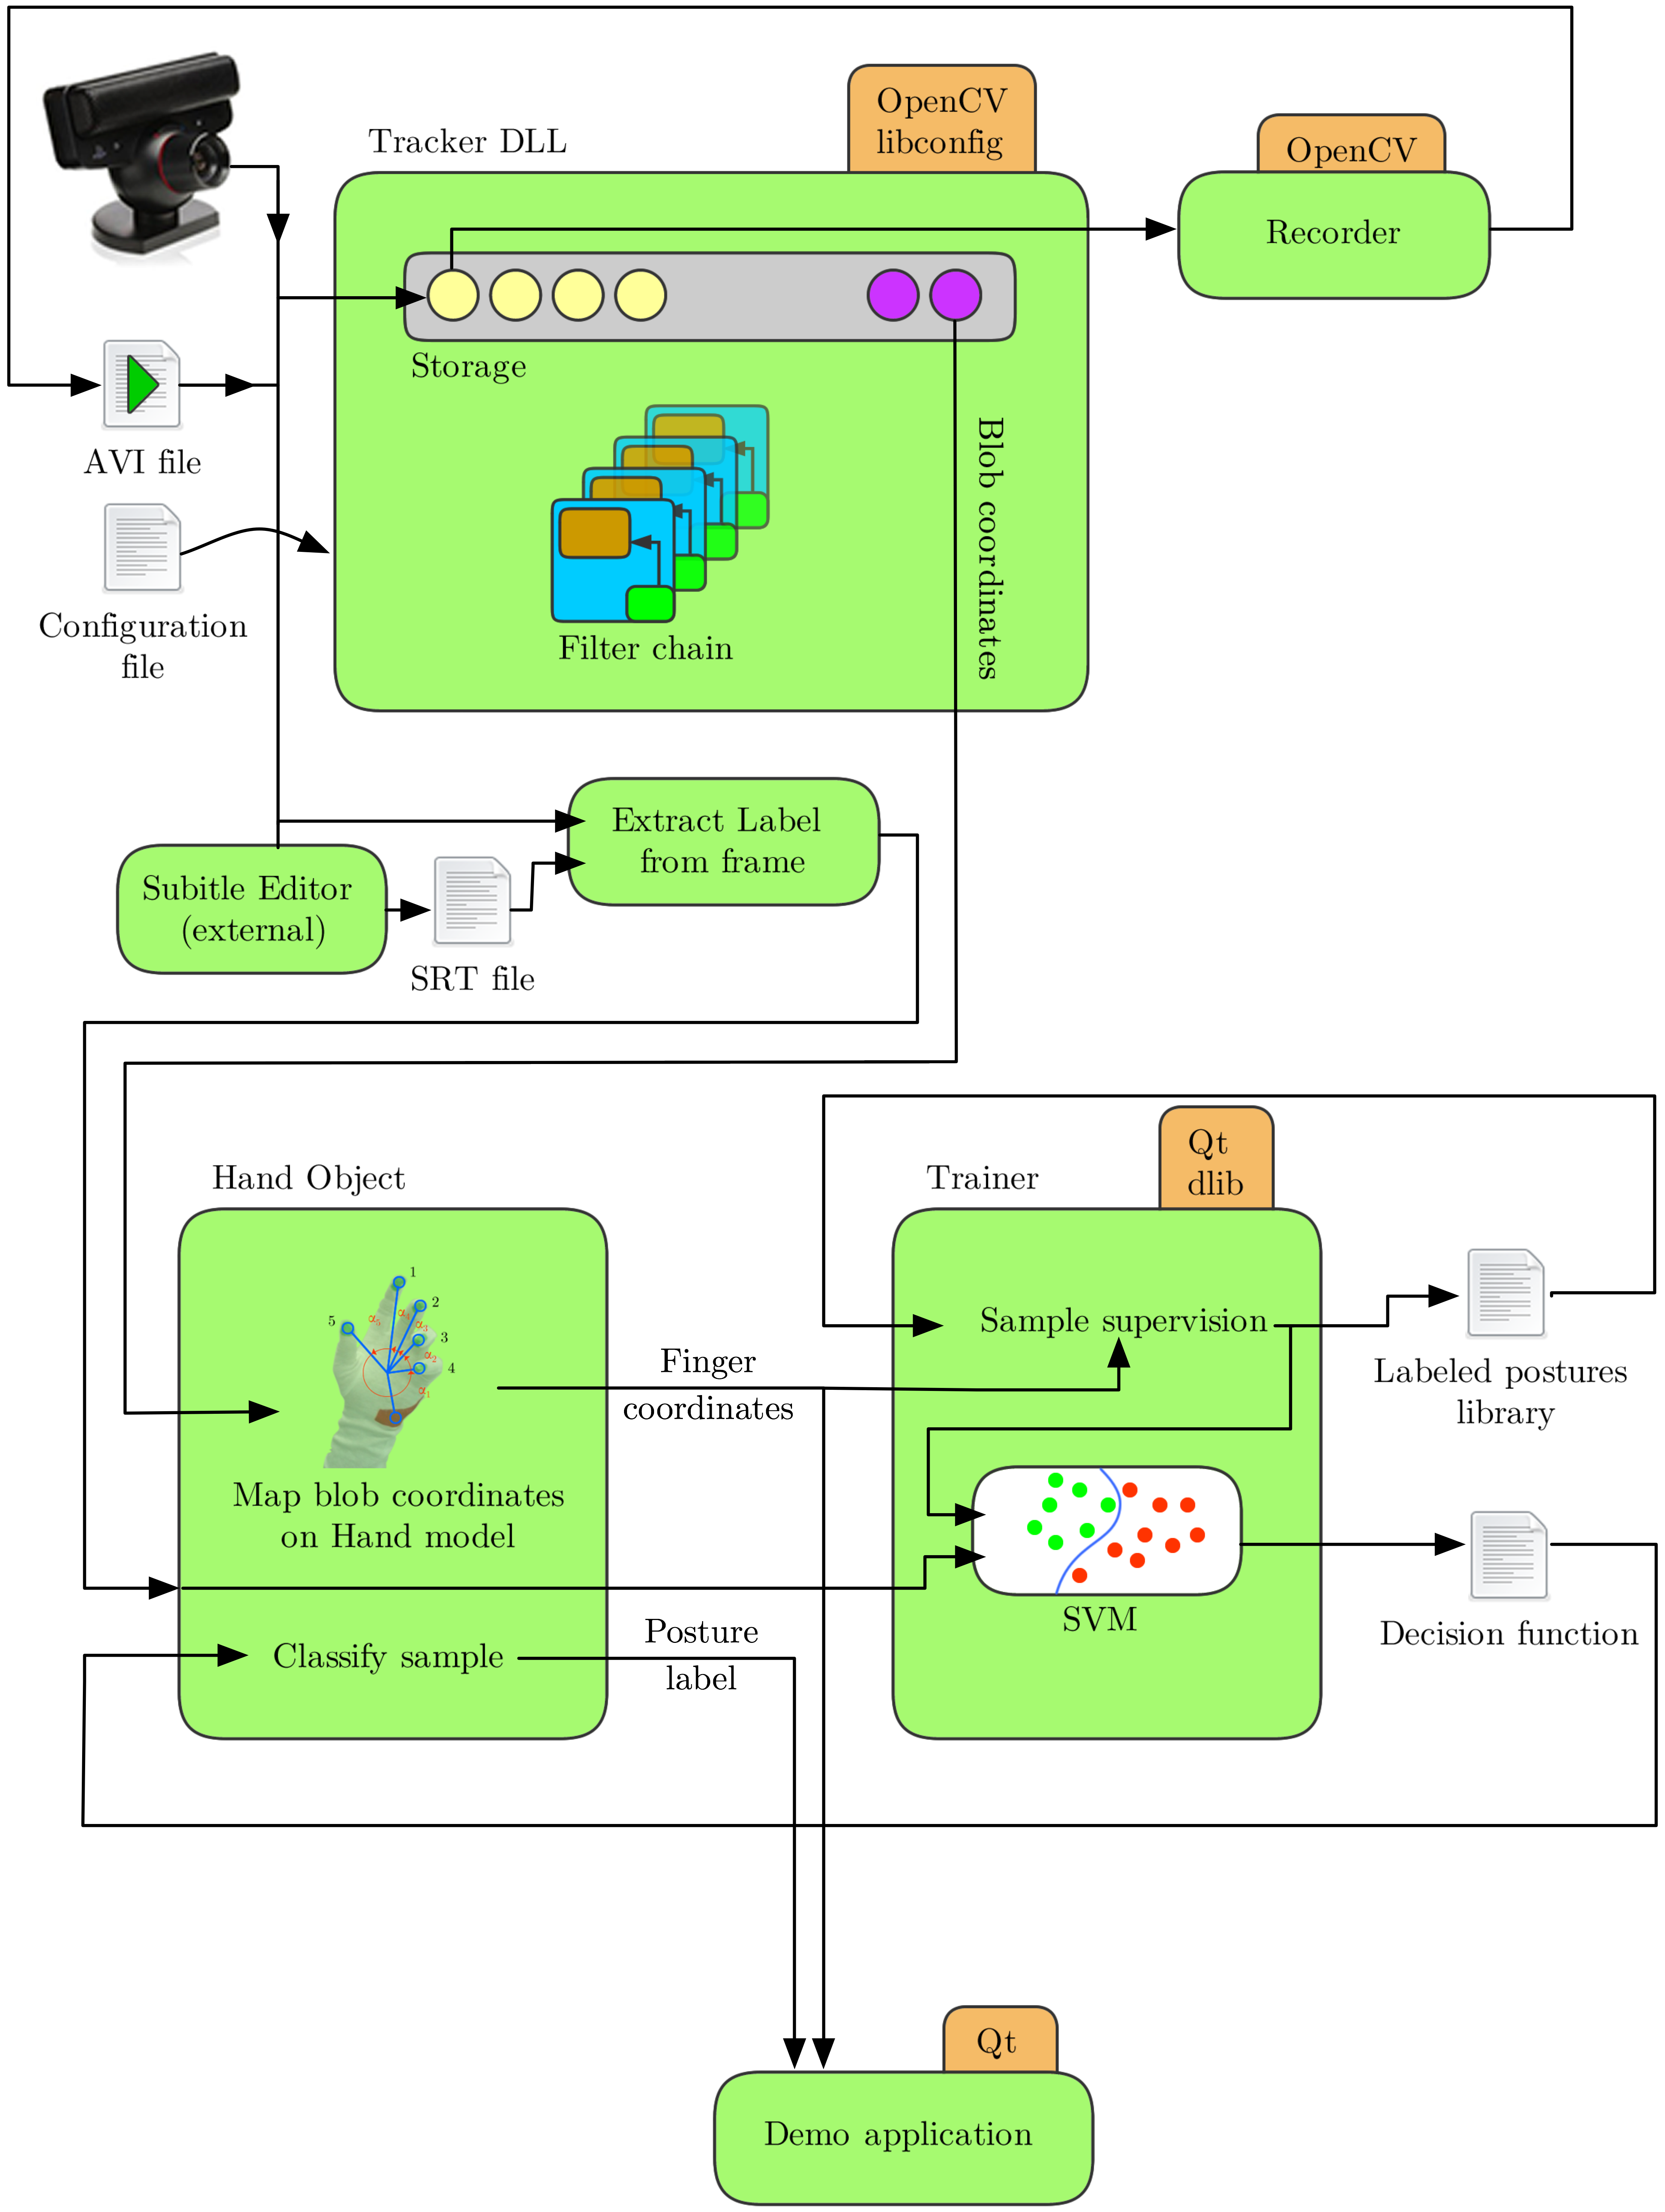
\includegraphics[width=1\textwidth]{images/arch} 
\caption{General architecture of the Ergonomic Gestures Recognition system}
\label{fig:architecture}
\end{figure}

%%%-%-%-%-%-%-%-%-%-%-%-%%-%-%-%-%-%-%-%-%-%-%-%%%
\section{Tracker configuration}
\label{sec:tracker-configuration}

The tracker module is implemented as a library that can be dynamically linked from an another program. This tracker is optimized for speed: it has to run several image processing filters for each frame and achieve a reasonable frame-rate of 10 to 30 FPS. However the frame-rate depends entirely on the optimizations of each image processing algorithm.

The tracker consists of three parts: a storage object, a filter chain and a camera thread. The camera thread acquires the images from the PS3 Eye camera at 60 frames per second in a separate thread. 

The storage object is a simple key-value storage, or more precisely a "key-anything" storage. Its only purpose is to eliminate the need to supervise each allocation and release of memory for the images at each iteration of the filter chain. It has also locking mechanisms implemented to ensure data consistency when an external thread accesses the memory in the storage object. The storage object is accessible from everywhere in the tracker: for example in the initialization phase, the camera descriptors are stored in it, but each image processing algorithm can also access it for its own purposes.

%------------------------------------------------%
\subsection{Filter chain}
\label{sub:filter-chain}

The filter chain allows an arbitrary configuration on how the image processing algorithms are linked. Each element in the chain, called step, can have one image processing algorithm, called filter, associated to it.
Each step has also an overlay object, that can, whenever it is displayed, adjust the parameters and specify the input images of the filter. The filter object itself declares how many input images it needs, and upon executing its function returns a result image. These resulting images can now be used as input images, or sources, to each filter (see figure \ref{fig:chain-general}).

\begin{figure}[H]
\center
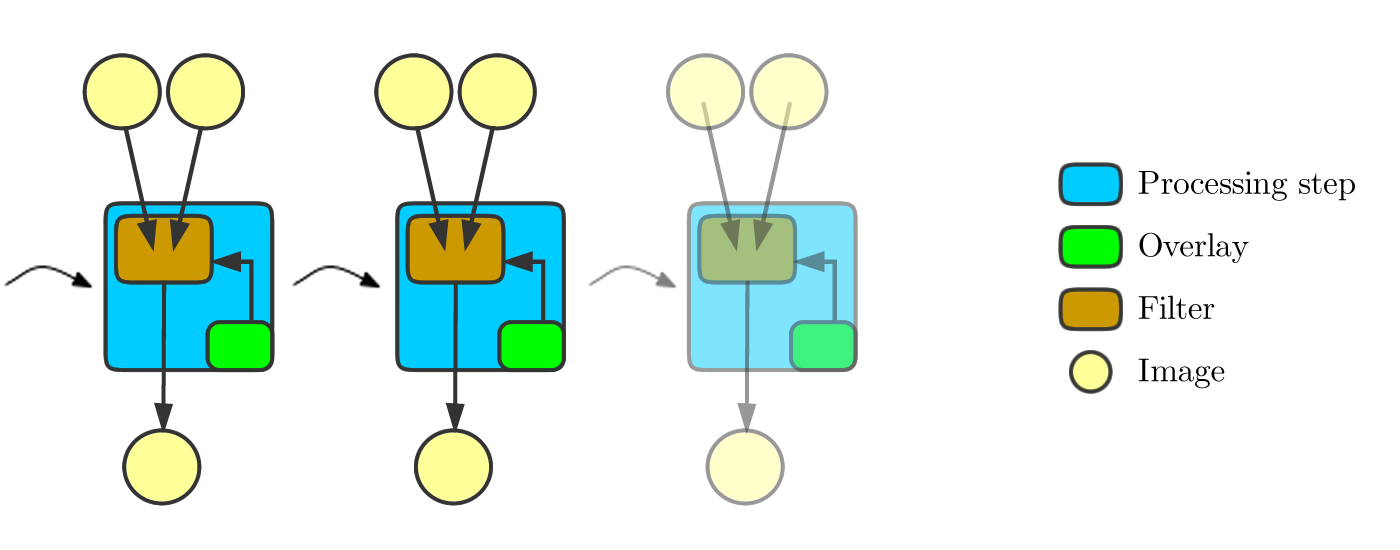
\includegraphics[width=0.9\textwidth]{images/steps} 
\caption{Image processing chain with reconfigurable processing steps: the filter and source image(s) can be specified using the overlay object belonging to the step. }
\label{fig:chain-general}
\end{figure}

The execution of the filter chain is sequential, but the specification of the input sources allow an arbitrary and reconfigurable order of image processing operations. 
To improve the execution speed, there is no GUI control elements used from QT or the built-in OpenCV GUI controls. Instead the user interface is directly in overlay mode with the result image of the selected step (see figure \ref{fig:lab-overlay}).

\begin{figure}[H]
\center
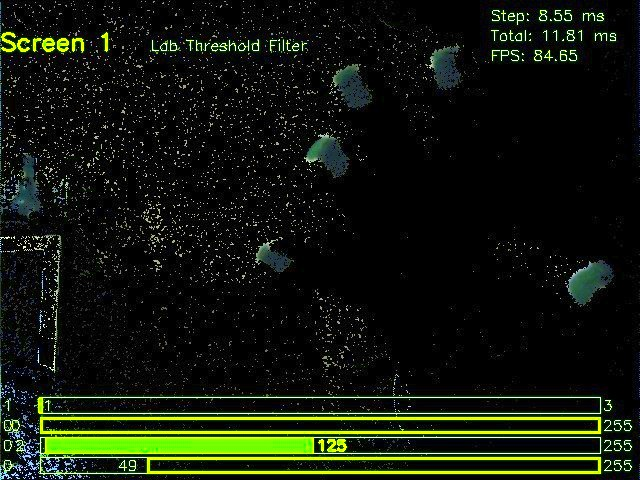
\includegraphics[width=0.7\textwidth]{images/step_lab} 
\caption{Lab threshold filter with overlay interface}
\label{fig:lab-overlay}
\end{figure}

As mentioned in \ref{sec:tracker-configuration}, each filter has access to the global storage object, and can store temporary images in it, but also other objects like vectors containing the positions of the detected blobs. Knowing the identifying key to this vector of points, an external program linked to the tracker DLL can retrieve this information.

%------------------------------------------------%
\subsection{Image processing filters}
\label{sub:image-processing-filters}

The tracker provides a small but easily extensible list of filters:
\begin{itemize}
\item Lab threshold: convert from the RGB color space to the Lab color space, and threshold each plane with a value range.
\item RGB threshold: threshold each RGB plane with a value range.
\item Binary threshold: converts an image into a gray image if needed, and performs a binary threshold.
\item Erosion: convolution directly implemented in OpenCV with a 3$\times$3 kernel.
\item Dilation: convolution directly implemented in OpenCV with a 3$\times$3 kernel.
\item Gaussian smooth: : convolution directly implemented in OpenCV with a gaussian kernel.
\item Add: overlays non-zero parts of a first source image onto a second source image.
\item Blob detection (see below)
\item Fast corner detection (see below)
\end{itemize}

The blob detection and the fast corner detection filters use external algorithms, but the others are implemented with OpenCV functions. The blob detection filter uses the cvBlobsLib available at the OpenCV Wiki \cite{cvblobslib}. The blob detection itself is based on the linear-time component labeling algorithm using contour tracing technique by Chang et al. \cite{blobs}. Tests have shown, that this algorithm performs well, as long the number of blobs remains small. However when the color thresholding filter and the erosion filter leave enough noise in the resulting image, the blob detection algorithm takes up to a second and thus impeaching the fast real-time execution. 
In order to circumvent this possible delay, other detection algorithms were investigated. The most promising was the FAST corner detection algorithm from Rosten and Drummond \cite{fast, fast2}. This algorithm is capable of detecting corners at the same speed with noisy and clear images. However this approach was not continued, because the interpretation of the found corners would take more time than the blob detection filter.

%\subsubsection{Lab threshold filter}
%Each filter has to implement a filter function which takes a vector of images as arguments and return an image. Additionally, the constructor has to declare the parameters that can be adjusted in the overlay and a cloning function that ensures the filter is instantiated correctly. 

\subsection{Chosen filter chain}
\label{sub:chosen-filter-chain}

In this project three consecutive operations for each marker color of the glove (red and green) were empirically selected (see figure \ref{fig:chain-specific}):
\begin{enumerate}
\item Lab Threshold filter
\item Erosion filter
\item Blob detection
\end{enumerate} 

\begin{figure}[H]
\center
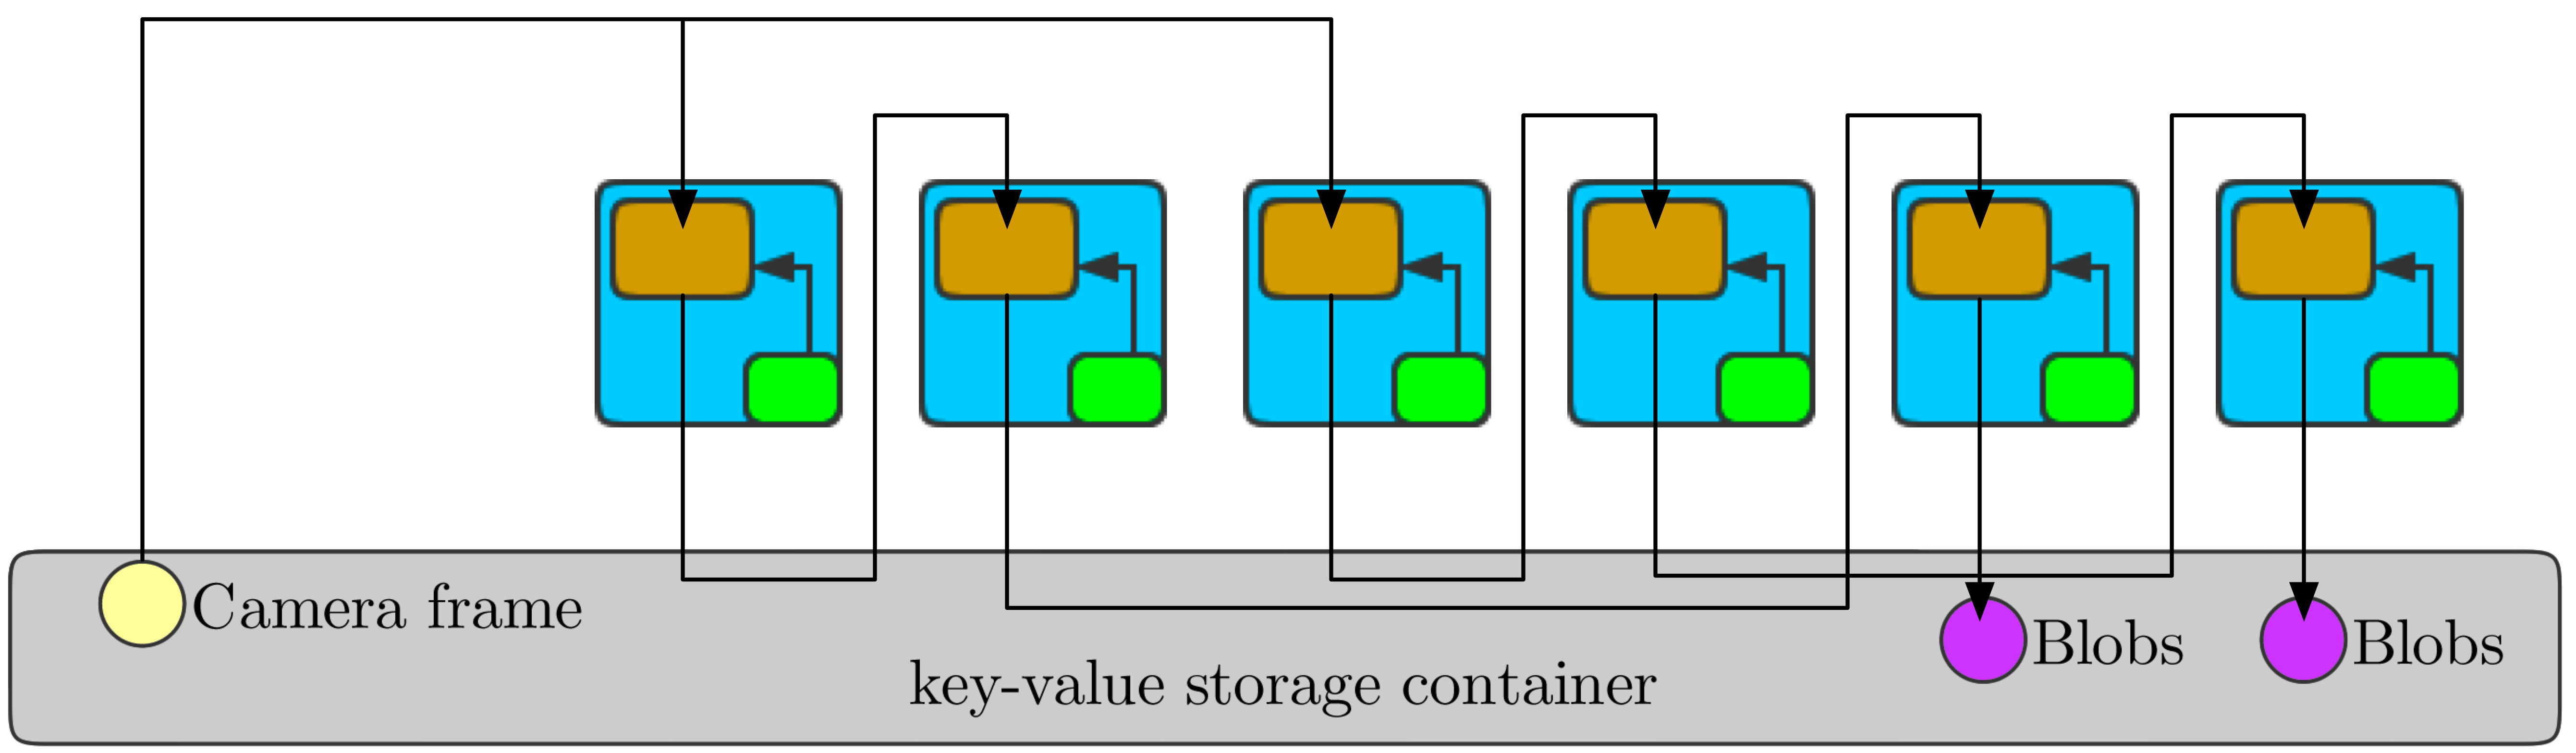
\includegraphics[width=0.8\textwidth]{images/steps_egr} 
\caption{Specific chain used in this project: sequential execution order independent of input/output cross linking. Each output image is automatically stored in the global storage but filters can specify additional storage objects (like a vector of blob coordinates)}
\label{fig:chain-specific}
\end{figure}

The six image processing algorithms could run on an average of 25 frames per second on a Macbook with an Intel Core Duo at 2.5 Ghz, and with a PS3 Eye camera providing 640$\times$480 pixels frames at 60 frames per second. Initially the tracker loop was slightly faster, but had no locking mechanisms on the storage object. Counterintuitively, without locking mechanisms used the CPU up to 90\% with an average of 29 frames per second, but with locking mechanisms the CPU utilization averaged at 45\% and 25 frames per second.
However the locking mechanisms were indispensable: without them random crashes occurred frequently. 

The following table presents the filter chain CPU utilization in milliseconds:

\begin{table}[h]
\caption{Filter processing times}
\tablestyle
\begin{tabular}{*{2}{v{0.3\textwidth}}}
\toprule
   \tablehead Filter &
   \tablehead Processing time \tabularnewline
\midrule
Lab threshold filter (green) & 9.7 ms \tabularnewline
Erosion filter (green) &  1.5 ms \tabularnewline
Blob detection (green) & 6.6 ms \tabularnewline
Lab threshold filter (red) & 9.8 ms \tabularnewline
Erosion filter (red) & 1.2 ms \tabularnewline
Blob detection (red) & 5.5 ms \tabularnewline
Add filter & 1.5 ms \tabularnewline
Add filter & 0.4 ms \tabularnewline
Tracker overhead & 2.1 ms \tabularnewline
\bottomrule
\textbf{Total} & \textbf{38.3 ms} \tabularnewline
\bottomrule
\end{tabular}
\label{tbl:filters-time}
\end{table}

The resulting filtered images of this specific filter chain are presented in chapter \ref{chap:evaluation} (see figure \ref{fig:tracker-chain}).

%%%-%-%-%-%-%-%-%-%-%-%-%%-%-%-%-%-%-%-%-%-%-%-%%%
\section{Model mapping}
\label{sec:model-mapping}

The model mapping is a step in gesture recognition that is not always necessary, depending on the recognition process. But it is helping to accumulate information gathered from the tracker in a structured way, eventually with some transformations applied, in order to exploit physical constraints of the hand. 
In this project, several simple physical constraints are implemented, but the model of the hand could implement more complex constraints, like generalised constraints for the degrees of freedom for the fingers or the distinction of the left and right hand.

%------------------------------------------------%
\subsection{Hand model}
\label{sub:hand-model}

In chapter \ref{chap:chosen-gestures} the interface control gestures of pointing, pinching (zoom) and swiping were chosen. These can be decomposed in the following distinct postures:
\begin{itemize}
\item Pointing posture
\item Pinching posture
\item Posture with all the fingers on the left side (part of the swiping gesture)
\item Posture with all the fingers on the right side (part of the swiping gesture)
\end{itemize}

\begin{figure}[H]
	\centering
	\subfloat[Pointing]{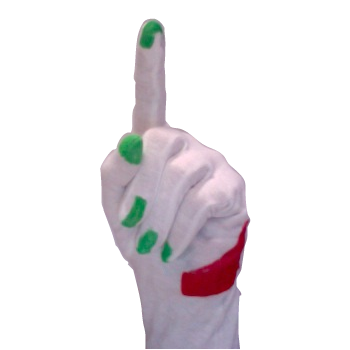
\includegraphics[width=0.22\textwidth]{images/hand_pointing}}
	\hspace{0.03\textwidth}
	\subfloat[Pinching]{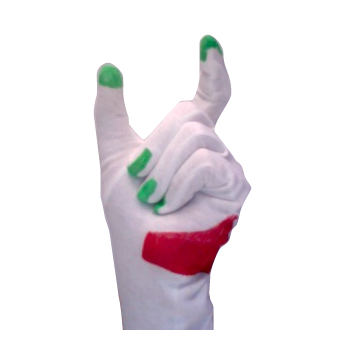
\includegraphics[width=0.22\textwidth]{images/hand_zooming}}
	\hspace{0.03\textwidth}
	\subfloat[Fingers left]{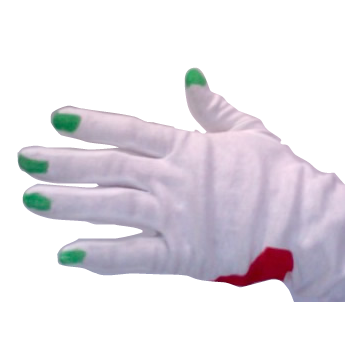
\includegraphics[width=0.22\textwidth]{images/hand_left}}
	\hspace{0.03\textwidth}
	\subfloat[Fingers right]{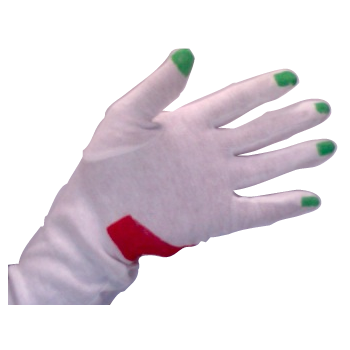
\includegraphics[width=0.22\textwidth]{images/hand_right}}
	\caption{Postures of hand with glove}
	\label{fig:glove-postures}
\end{figure}

The hand model should adhere to the following simple generalisations:

\begin{itemize}
\item A hand has five fingers.
\item A hand has one wrist.
\item Though crossing of fingers is physically possible, it is not very natural and easy to do: there is a circular order of the fingers and the model asserts that it remains (mostly) constant.
\item The index finger and the thumb are the most articulated fingers, while the little finger, the ring finger, and sometimes the middle finger follow the same motion patterns (synchronously): the positions of the little finger and the ring finger can be estimated together.
\end{itemize}

A hand model constructed according to these generalisations should at least contain the following properties:
\begin{itemize}
\item Five finger coordinates
\item Wrist coordinate
\item Order to the fingers: index finger follows the middle finger, thumb follows the index finger
\item Velocity vectors of fingers and wrist
\end{itemize}

%------------------------------------------------%
\subsection{Mapping}
\label{sub:mapping}

To map the unordered vector of finger coordinates and the wrist coordinates obtained from the tracker to the model described in \ref{sub:hand-model}, several mechanisms involving prediction of the coordinates for the next frame, along with an algorithm that finds the best permutation of recognized fingers to the prediction of the previous finger coordinates have been investigated. But the most robust mapping followed the generalization property, that the fingers have a specific order: once the index finger has been identified, the next fingers are mapped according to a circular path along the mass center of all the points (see figure \ref{fig:hand-model}):

\begin{enumerate}
\item Calulate mass center of all points. The wrist has double wheight.
\item Calculate angles $\alpha_{1\ldots n}$ of the vectors from the mass center to each finger coordinate.
\item Sort the fingers according to this angle $\alpha_{1\ldots n}$ in descending order.
\item Cycle the finger vectors in order to position the index finger as the first finger.
\item Missing fingers are calculated as an average of all the fingers without index finger and thumb (first and last finger of the fingers vector).
\end{enumerate}

\begin{figure}[H]
\center
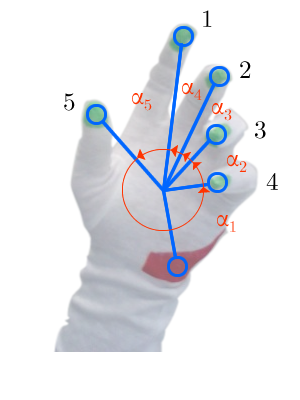
\includegraphics[width=0.275\textwidth]{images/hand-model} 
\caption{Glove with overlayed hand model. $\alpha_{1\ldots n}$ indicates the angle of the vectors from the mass center to each finger coordinate. }
\label{fig:hand-model}
\end{figure}

%%%-%-%-%-%-%-%-%-%-%-%-%%-%-%-%-%-%-%-%-%-%-%-%%%
\section{Training and classification}
\label{sec:training-and-classification}

Initially, attempts were made to directly classify the gesture using a Hidden Markov Model (HMM) as classifier and the set of coordinates of the fingers, or alternatively some other features best describing the gesture in question, as input of this classifier. For this, a test program was implemented, where different features of gesture could be temporally inspected: beside the coordinates, a feature that look promising was the distance of each finger to the wrist or the mass center. This length would also, in a general way, characterize the contraction of the finger, reducing the degree of freedom of each finger in a physical, two-dimensional model to one.

However, it became clear that even if this approach would eventually work, it still was not viable for real-time control gestures. Imagine a scenario where a trained classifier was fed with samples of finger coordinates for each new frame. Two common problems of gesture recognition would arise: when does a gesture begin, and when does it end? But assuming these key moments could somehow be identified, the HMM would still only classify the gesture correctly at its end. At a closer inspection of the gestures defined in section \ref{sec:gestures}, it appeared, that the interface needed to know that the user was pointing somewhere, as soon the he entered a key posture (namely the pointing posture). Equally, as soon the user would stop pointing, the interface does not need to update a cursor position. This led to another approach, which follows more closely the definition of gestures being a sequence of postures.

The recognition approach implemented in this project consists of two parts: 
\begin{enumerate}
\item Posture training and classification from finger coordinates
\item Gesture classification from posture sequences.
\end{enumerate}
This separation allows real-time interaction, as posture classification is frame-based and could have an effect on the interface nearly instantaneously, whereas gestures are time-dependent and require several frames to take effect.

%------------------------------------------------%
\subsection{Sample collection}
\label{sub:sample-collection}

The process of sample collection requires one or more recorded videos containing sequences of postures selected in section \ref{sub:hand-model} and conforming to the constraints of section \ref{sub:environmental-constraints}. Additionally, a way of pre-labeling the postures semi-automatically was put in place, which eliminated the need of manually labeling each posture. This was not strictly necessary, but helped substantially for labeling one minute of video: 60 seconds $\times$ 25 frames per second results in 1500 frames, or approximately 1200 usable postures. The pre-labeling process included a file for the labels, which consisted in a simple text-based subtitle file. This subtitle file had the advantage that it could be edited in any subtitle editor (see figure \ref{fig:subtitle-editor}). The combination of a video and its subtitle file containing the labels of postures makes it also possible to view and inspect the posture-label mapping in any video player capable of displaying subtitles. With this pre-labeling technique the process of sample collection consisted of:

\begin{enumerate}
\item Roughly pre-label postures in a video with a subtitle editor, resulting in a SRT subtitle file,
\item Set the video as the source of the tracker,
\item Map the resulting blobs to a hand model and label it according to the corresponding frame in the subtitle file (see figure \ref{fig:collect-samples}),
\item Save the supervised collection of labeled postures to a posture database file.
\end{enumerate}

\begin{figure}[H]
\center
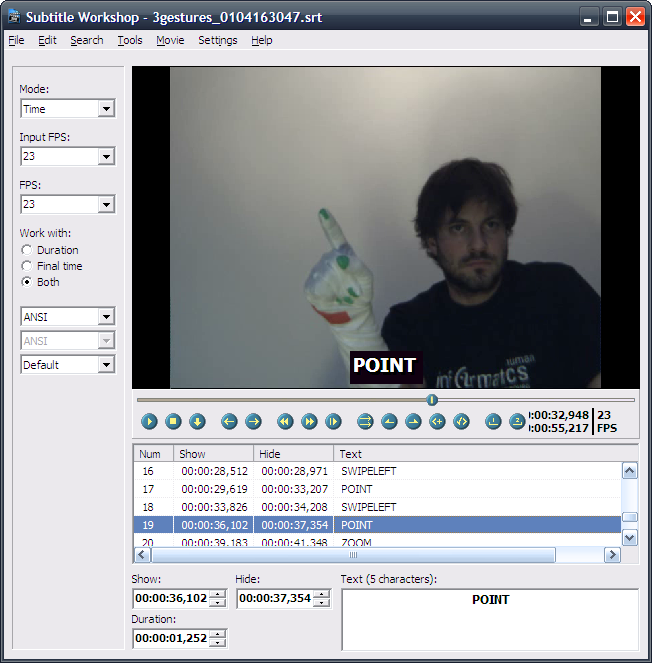
\includegraphics[width=0.67\textwidth]{images/subtitle-editor} 
\caption{Posture labeling with an external subtitle editor. Each posture is labeled with the beginning and the end (in ms) of its presence in the video sequence. This demarcation is the basic structure of a subtitle file. }
\label{fig:subtitle-editor}
\end{figure}

\begin{figure}[H]
\center
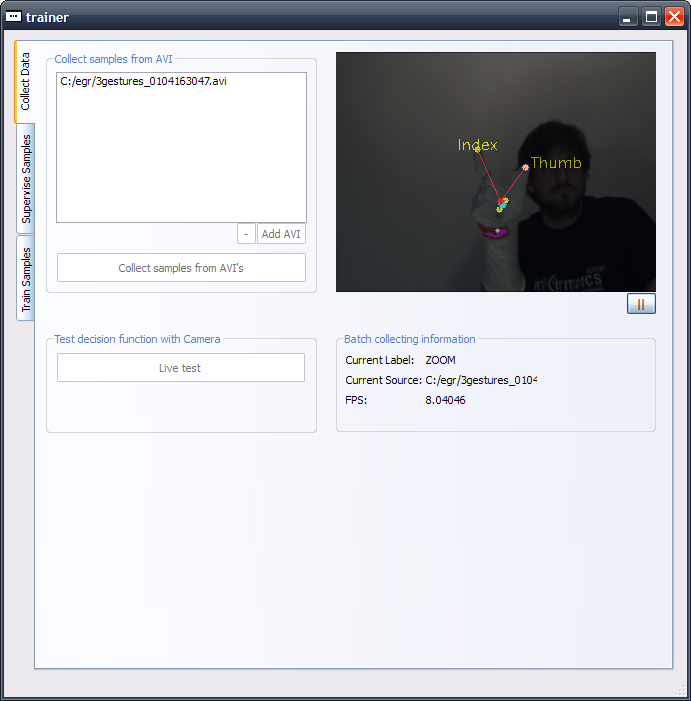
\includegraphics[width=0.67\textwidth]{images/collect-samples} 
\caption{Posture sample collection}
\label{fig:collect-samples}
\end{figure}

%------------------------------------------------%
\subsection{Sample supervision}
\label{sub:sample-supervision}

In a first attempt a support vector machine was trained with the posture samples database obtained from section \ref{fig:collect-samples}. But even the parameter estimation for the support vector machine with a cross validation algorithm did not finish to run in days. At a closer inspection of the collected samples, it became apparent that some samples have been mislabeled, due to the rough boundary of beginning and end of a posture sequence obtained from the subtitle file. Other samples included unusable tracking results from background noise or occluded finger positions. In order to provide a correctly labeled sample database to a classifier, a graphical user interface for quick relabeling and posture inspection was implemented (see figure \ref{fig:sample-supervision}). It allowed to view only samples from one label class, relabel them, or remove the sample altogether from the database, due to inconsistent finger coordinates. In a filtered mode, where only one label class was visible, a cumulative view of all the finger positions in this label class was displayed, helping to inspect the overall finger coordinate distribution of this label class (see figure \ref{fig:cumulative-coordinates}). Each view of a sample displays the finger coordinates relative to the wrist position, giving a easily identifiable representation of a posture.

\begin{figure}[H]
\center
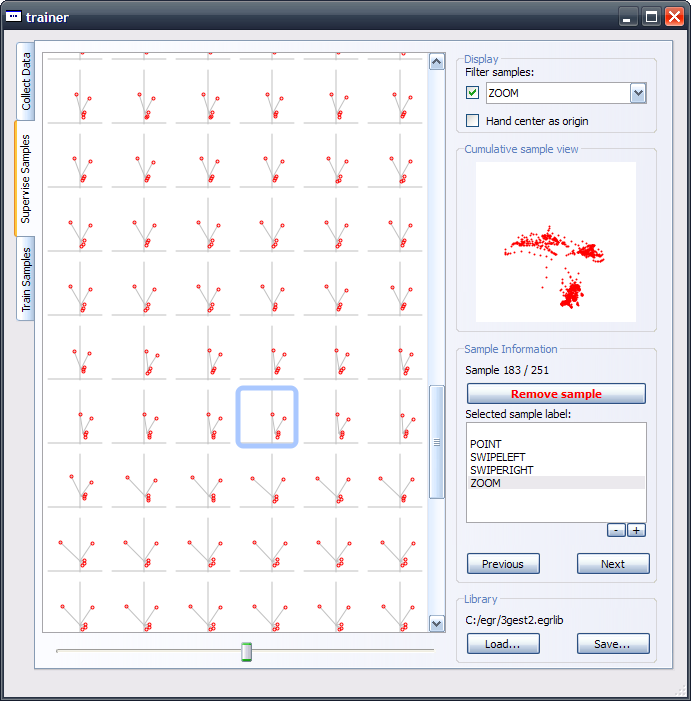
\includegraphics[width=0.67\textwidth]{images/sample-supervision} 
\caption{Sample supervision}
\label{fig:sample-supervision}
\end{figure}

\begin{figure}[H]
	\centering
	\subfloat[Pinching]{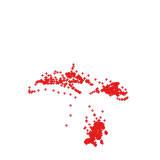
\includegraphics[width=0.18\textwidth]{images/allsamples-zoom}}
	\hspace{0.01\textwidth}
	\subfloat[Pointing]{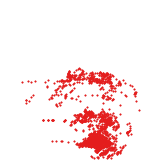
\includegraphics[width=0.18\textwidth]{images/allsamples-point}}
	\hspace{0.01\textwidth}
	\subfloat[Fingers on the left]{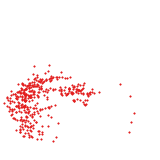
\includegraphics[width=0.18\textwidth]{images/allsamples-left}}
	\hspace{0.01\textwidth}
	\subfloat[Fingers on the right]{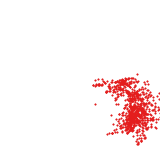
\includegraphics[width=0.18\textwidth]{images/allsamples-right}}
	\hspace{0.01\textwidth}
	\subfloat[Garbage]{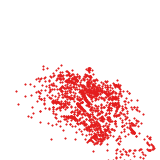
\includegraphics[width=0.18\textwidth]{images/allsamples-empty}}
	\caption{Cumulative view of finger positions for each label}
	\label{fig:cumulative-coordinates}
\end{figure}

%------------------------------------------------%
\subsection{Posture training}
\label{sub:posture-training}

The training of a classifier is done using the dlib C++ library, which packages many classification, regression and clustering algorithms in its machine learning module:
\begin{itemize}
\item Classification (binary): Relevance Vector Machine (RVM), C-Support Vector Machine (C-SVM), C-SVM using empirical kernel maps, linear C-SVM, $\nu$-SVM, Pegasos-SVM
\item Regression: Kernel Recursive Least Squares (KRLS), Kernel Ridge Regression (KRR), Multilayer Perceptron (MLP), $\epsilon$ Support Vector Regression ($\epsilon$-SVR)
\item Kernels: linear kernel, polynomial kernel, radial basis function kernel, sigmoid kernel
\end{itemize}

For this project a multi-class $\nu$-SVM will be used to train a decision function, in order to distinguish between the different classes of postures. A non-linear support vector machine with a kernel function  is ideally suited for this task: a support vector machine separates a set of objects using a linear boundary, or decision plane. However not every classification problem is linearly separable: but the kernel function can rearrange, or transform the objects in a higher-dimensional space, known as feature-space, so that a hyperplane in this higher-dimensional space can linearly separate these objects \cite{svmbook} (see figure \ref{fig:svm-boundary}).

\begin{figure}[H]
	\centering
	\subfloat[Non-linear decision boundary]{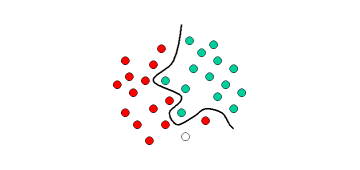
\includegraphics[scale=0.5]{images/svm1}}
	\hspace{0.03\textwidth}
	\subfloat[Linear decision boundary in feature space]{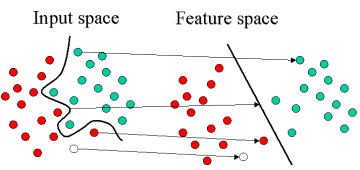
\includegraphics[scale=0.5]{images/svm2}}
	\caption{Example of a non-linearly separable classification \cite{svmbook}}
	\label{fig:svm-boundary}
\end{figure}

The feature vector $\textbf{v}$ used to train the $\nu$-SVM is a 10-dimensional vector containing the two-dimensional coordinates of the five fingers:
\[ \textbf{v} = \begin{pmatrix} x_1 \\ y_1 \\ \vdots \\ x_5 \\ y_5  \end{pmatrix} \]

The decision function is trained using a one versus one training structure: since the classifiers provided by dlib are binary classifiers, this structure creates for $n$ possible classes $\frac{n\cdot(n-1)}{2}$ binary classifiers to vote on the identity of a test sample. For the 4 possible postures defined in section \ref{sub:hand-model} there will be 5 classes, including a garbage posture representing everything not belonging to the other 4 postures.

This trained classifier produces a decision function that has an accuracy of 94\% on the training data.

%------------------------------------------------%
\subsection{Posture classification}
\label{sub:posture-classification}

In a cross-validation test the decision function obtained in section \ref{sub:posture-training} produces a confusion matrix, represented in table \ref{tbl:confusion}. This confusion matrix qualitatively gives an indication if the classifier will work on similar test samples. 

\begin{table}[h]
\caption{Confusion matrix of the trained decision function}
\tablestyle
\begin{tabular}{*{6}{v{0.12\textwidth}}}
\toprule
    Identified as: &
    Garbage &
    Pointing &
    Left &
    Right &
    Zoom \tabularnewline
\midrule
\tablehead Garbage & 283 & 11 & 8 & 12 & 3  \tabularnewline
\tablehead Pointing & 14 & 383 & 0 & 0 &0  \tabularnewline
\tablehead Left & 6 & 0 & 71 & 1 & 0 \tabularnewline
\tablehead Right & 8 & 0 & 0 & 166 & 0  \tabularnewline
\tablehead Zoom & 4 & 1 & 0 & 0 & 247  \tabularnewline

\bottomrule
\end{tabular}
\label{tbl:confusion}
\end{table}

In a live test with the camera, the accuracy is subjectively very good for the postures of pinching, with all the fingers on the left and with all the fingers on the right. However there are more misclassifications of the pointing posture, identified as a posture with all the fingers on the right. Going back to section \ref{sub:sample-supervision}, a simple comparison of the cumulative finger positions for each label class does not reveal large overlaying areas for the finger coordinates distribution of these postures (see dark regions in figure \ref{fig:cumulative-comparision}).

\begin{figure}[H]
	\centering
	\subfloat[Left (blue), garbage (orange), right (green)]{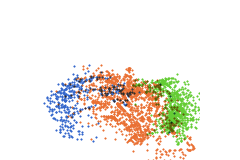
\includegraphics[scale=0.55]{images/allsamples-left-nothing-right}}
	\hspace{0.01\textwidth}
	\subfloat[Pointing (red), pinching (green)]{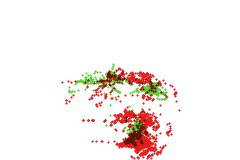
\includegraphics[scale=0.55]{images/allsamples-point-zoom}}
	\hspace{0.01\textwidth}
	\subfloat[Pointing (red), right (green)]{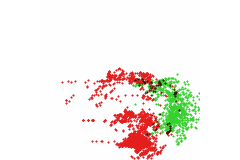
\includegraphics[scale=0.55]{images/allsamples-point-right}}

	\caption{Overlayed cumulative view of finger positions}
	\label{fig:cumulative-comparision}
\end{figure}

But these misclassifications can be filtered out with simple majority filter with a window size that is still acceptable for real-time posture classification. With a window size of 10 frames, which equals 0.4 seconds at 25 FPS, a majority can often be reached in 0.2 seconds, therefore providing a more robust posture classification, that still has a very low reaction time.

%------------------------------------------------%
\subsection{Gesture classification}
\label{sub:gesture-classification}

The recognition of a gesture can be achieved with an Hidden Markov Model (HMM) for each gesture. The state diagram for the pointing gesture (see figure \ref{fig:pointing-states}) has exactly the same structure as the zooming gesture, where there is only one state for the gesture and the only transition allowing to remain in that state is the key posture to this gesture. 

\begin{figure}[H]
	\centering
	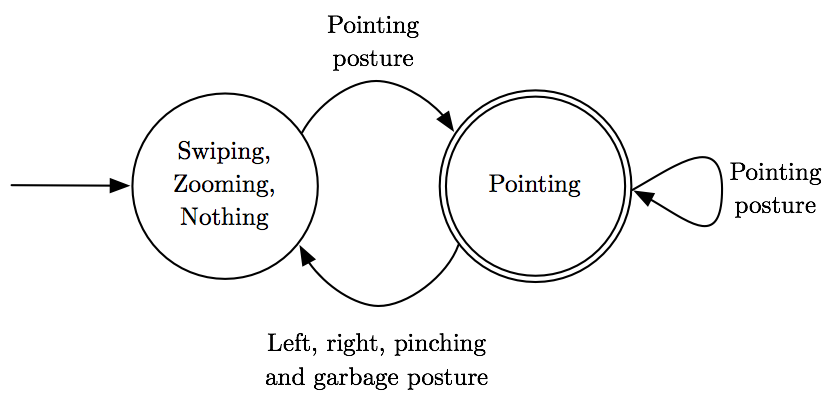
\includegraphics[width=0.5\textwidth]{images/states-pointing}
	\caption{State diagram of pointing gesture}
	\label{fig:pointing-states}
\end{figure}

The swiping gesture has a temporal dependency: the only way to reach the final swiping gesture state is to have  right postures follow left postures, or vice versa for a swiping gesture in the opposite direction (see figure \ref{fig:swiping-states}).
\begin{figure}[H]
	\centering
	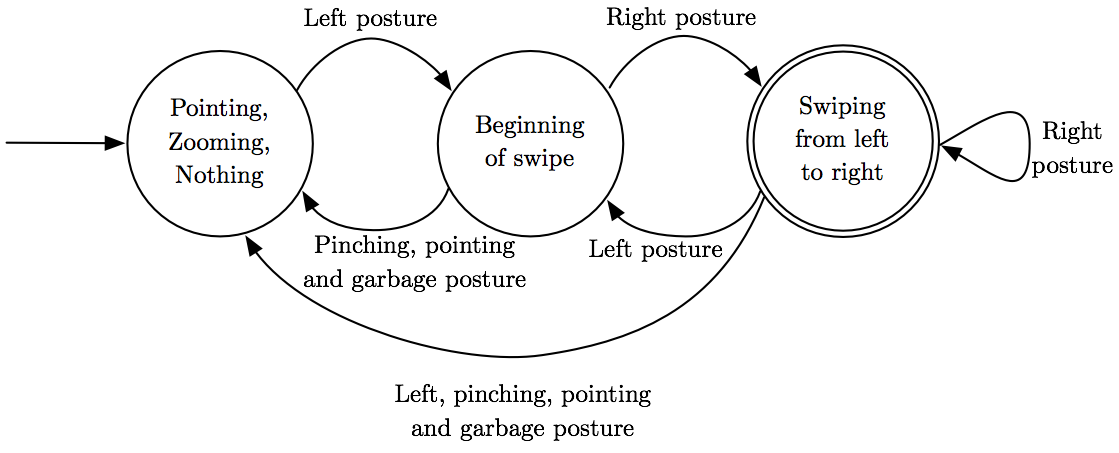
\includegraphics[width=0.7\textwidth]{images/states-swipe}
	\caption{State diagram of swiping (from left to right) gesture}
	\label{fig:swiping-states}
\end{figure}

These HMM's could be implemented using the HMM Toolkit \cite{htk}. But for the scope of this project and because of the low complexity of the gesture states the recognition was implemented programmatically without HMM's but respecting the transition logic of the gesture state diagrams.

However, gestures with more complex spatial or temporal dependencies would definitively require of the use of an appropriate structure like a HMM. As a simple example, a gesture with more complex spatial dependencies would be a certain hand posture, i.e. the pointing posture, following a specific trajectory, i.e. a circle, that has a symbolic meaning and is not used for the direct control of a cursor following this trajectory. The feature vector for this specific HMM would not only require the posture label, but also the coordinates of the normalized index finger position.
